\documentclass{article}
\usepackage[utf8]{inputenc}
\usepackage[russian]{babel}
\usepackage{amsthm}
\usepackage{amssymb}
\usepackage[a1paper]{geometry}
\geometry{papersize={29.7 cm, 25.0 cm}}
% \usepackage{tikz}
\usepackage{textcomp}
% \usepackage{marvosym}
% \usepackage{ esint }
\usepackage{graphicx}\usepackage{amsfonts}
\setlength{\topmargin}{-0.5in}
\setlength{\textheight}{8.1in}
\setlength{\oddsidemargin}{-0.4in}
\setlength{\evensidemargin}{-0.4in}
\setlength{\textwidth}{7in}
\setlength{\parindent}{0ex}
\setlength{\parskip}{1ex}
\title{Полный анализ функции}\begin{document}

\maketitle
\renewcommand{\abstractname}{Введение}\begin{abstract}Данный документ содержит полный анализ функции с разложением в ряд Тейлора, построением графика и взятием полной производной.\end{abstract}
\section*{Исходная функция.}

$f(x, z, y) = {{\ln{({x} + {z})}} \cdot {({3} + {y})}}$

\section{Взятие 1-ой производной по x.}

$ f(x) = {{\ln{({x} + {z})}} \cdot {({3} + {y})}}$

Кто бы мог подумать что:

${({{\ln{({x} + {z})}} \cdot {({3} + {y})}})}^{'} = {({\ln{({x} + {z})}})}^{'}\cdot {{3} + {y}} + {\ln{({x} + {z})}}\cdot {({{3} + {y}})}^{'}$

Можно убедиться, что:

${({{3} + {y}})}^{'} = {({3})}^{'} + {({y})}^{'}$

Заметим, что:

${({y})}^{'} = 0$

Не требует дальнейших комментариев:

${({3})}^{'} = 0$

Заметим, что:

${({\ln{({x} + {z})}})}^{'} = {{{({{x} + {z}})}^{'} } \over {{{x} + {z}}}}$

Кто бы мог подумать что:

${({{x} + {z}})}^{'} = {({x})}^{'} + {({z})}^{'}$

Нетрудно заметить:

${({z})}^{'} = 0$

Увидим, что:

${({x})}^{'} = 1$

Получаем:

$ f^{(1)}(x) = {{{{({1} + {0})} \over {({x} + {z})}} \cdot {({3} + {y})}} + {{\ln{({x} + {z})}} \cdot {({0} + {0})}}}$

\section{Упрощение.}

${{{{({1} + {0})} \over {({x} + {z})}} \cdot {({3} + {y})}} + {{\ln{({x} + {z})}} \cdot {({0} + {0})}}} = {{{1} \over {({x} + {z})}} \cdot {({3} + {y})}}$
\section{Вычисление значения функции в точке.}

$ f(100) = 32.5777 $
\section{Вычисление производной функции в точке.}

$ f^{'}(5) = 0.7 $
\section{Разложение данной функции в ряд Тейлора.}

${{\ln{({x} + {z})}} \cdot {({3} + {y})}} =  11.2661 + \frac{1.4}{1}\cdot x^1 - \frac{0.28}{2}\cdot x^2 + \frac{0.112}{6}\cdot x^3 - \frac{0.0672}{24}\cdot x^4 + \frac{0.05376}{120}\cdot x^5 - \frac{0.05376}{720}\cdot x^6 + \frac{0.064512}{5040}\cdot x^7 + o(x^7) $
\section{Взятие полной производной}

$F(x, z, y) = \sqrt{({{{1} \over {({x} + {z})}} \cdot {({3} + {y})}} \cdot \Delta x)^2 + ({{{1} \over {({x} + {z})}} \cdot {({3} + {y})}} \cdot \Delta z)^2 + ({\ln{({x} + {z})}} \cdot \Delta y)^2} $

\section{Уравнение касательной функции в точке x = 2.}

g(x) = $1 \cdot  x + 11.6214 $
\section{График функции и касательной к ней.}


\begin{figure}[ht]
\center
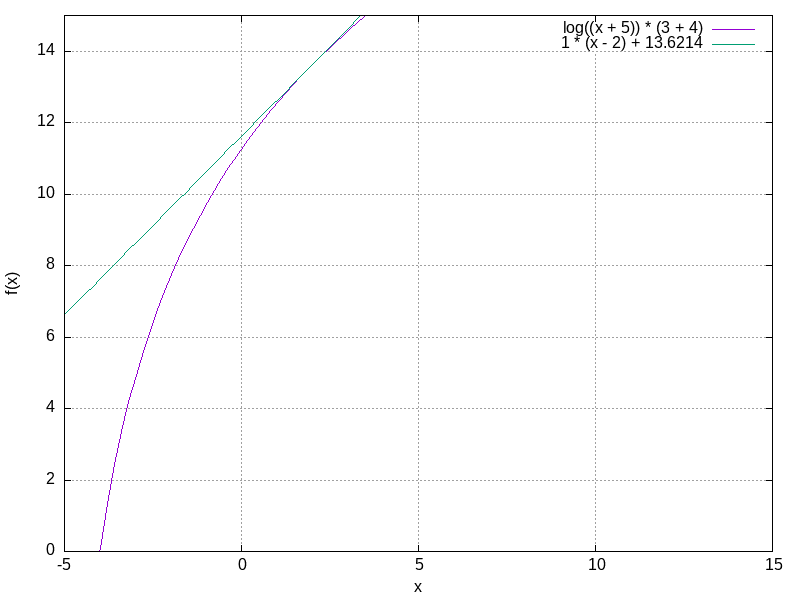
\includegraphics[scale=0.65]{graph.png}
\end{figure}
\end{document}